\chapter{Resultados y discusión} \label{chap:Resultados}
\chapterimage{figuras/ImagenesPortada/PortadaResultados.jpg}
\hrule
\vspace{3mm}

En este capítulo se detallan los resultados conseguidos con la versión final del brazo robótico.


\section{Resultados}
	
	El \textbf{espacio de trabajo} visto en el capítulo \ref{chap:Cinematica} representa las limitaciones matemáticas del sistema tal y como se ha planteado; además de la matemática, para definir el espacio de trabajo definitivo se deben tener en cuenta ciertas limitaciones impuestas por los mecanismos tal y como están construidos así como la compensación por muelles. El resultado de la última versión se puede ver en la figura \ref{fig:Resultados:workspace} con un rango de movimiento algo inferior a 50cm en el eje X y algo menor a 90cm en el eje Z. Se debe recordar que en la primera articulación no existe ninguna limitación mecánica ni de compensación, por lo que el rango de 180 grados establecido anteriormente permanece vigente.
	\\
	
	Aunque se considera que esta capacidad de movimiento es suficiente para el propósito que se pretende dar, siempre puede modificarse a otro rango, desplazándolo o ampliándolo, reajustando la compensación de carga así como la matemática de la cinemática (variando el origen de la realimentación).
	
	\begin{figure}[t]
		\centering
		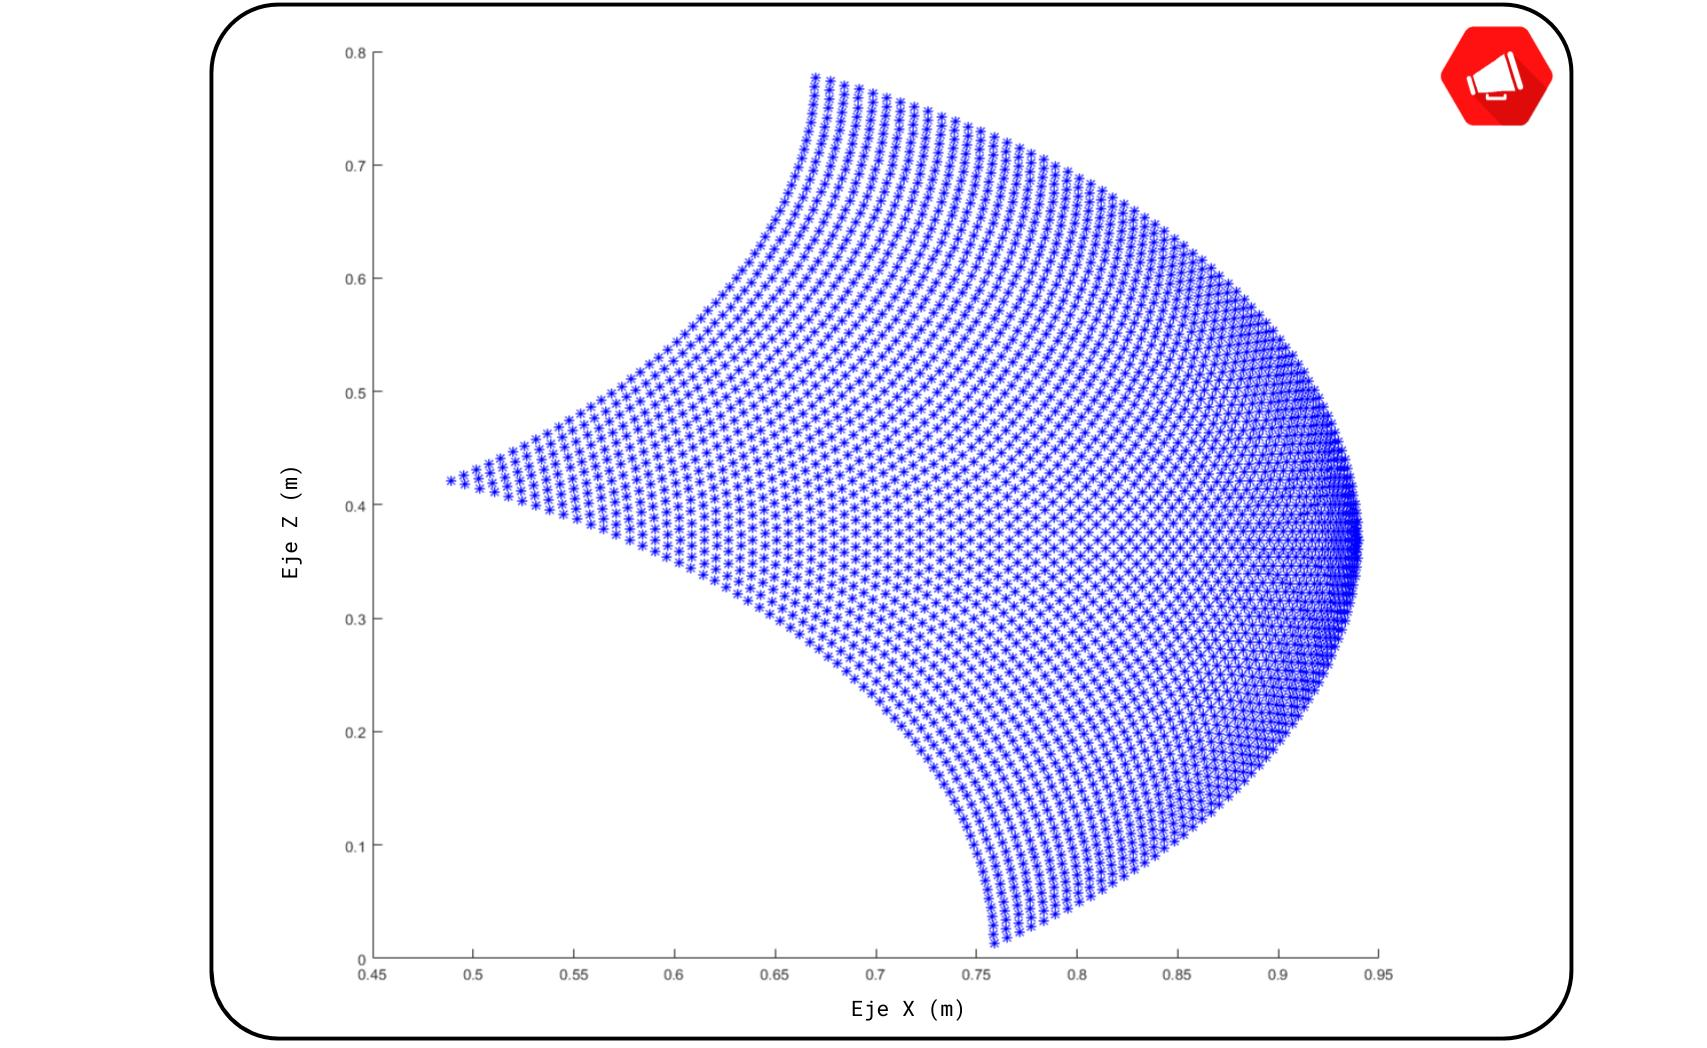
\includegraphics[width=1\textwidth]{figuras/Imagenes_Resultados/workspace_robot_real.jpg}
		\caption{Espacio de trabajo limitado por los muelles y la estructura mecánica}
		\label{fig:Resultados:workspace}
		\immagesource{Autor}
	\end{figure}
	
	Se ha conseguido controlar el brazo con la \textbf{carga} inicialmente planteada, de 780g. En la configuración definitiva el brazo robótico es capaz de aguantar hasta 1kg de carga en el extremo de la forma esperada. Aunque no se ha probado, nuevamente variando la tensión de los muelles esta capacidad puede incrementarse notablemente.
	\\
	
	Se han llevado a cabo dos test de \textbf{precisión} del brazo robótico, pudiendo verse los resultados en las figuras \ref{fig:Resultados:prueba1} y \ref{fig:Resultados:prueba2}. El prototipo presenta una estructura mecánica compleja realizada con técnicas y materiales que no aseguran gran precisión, aún así se ha conseguido dotar al brazo robótico de una precisión suficiente para el uso para el cual será destinado. 
	\\
	
	\begin{figure}[t]
		\centering
		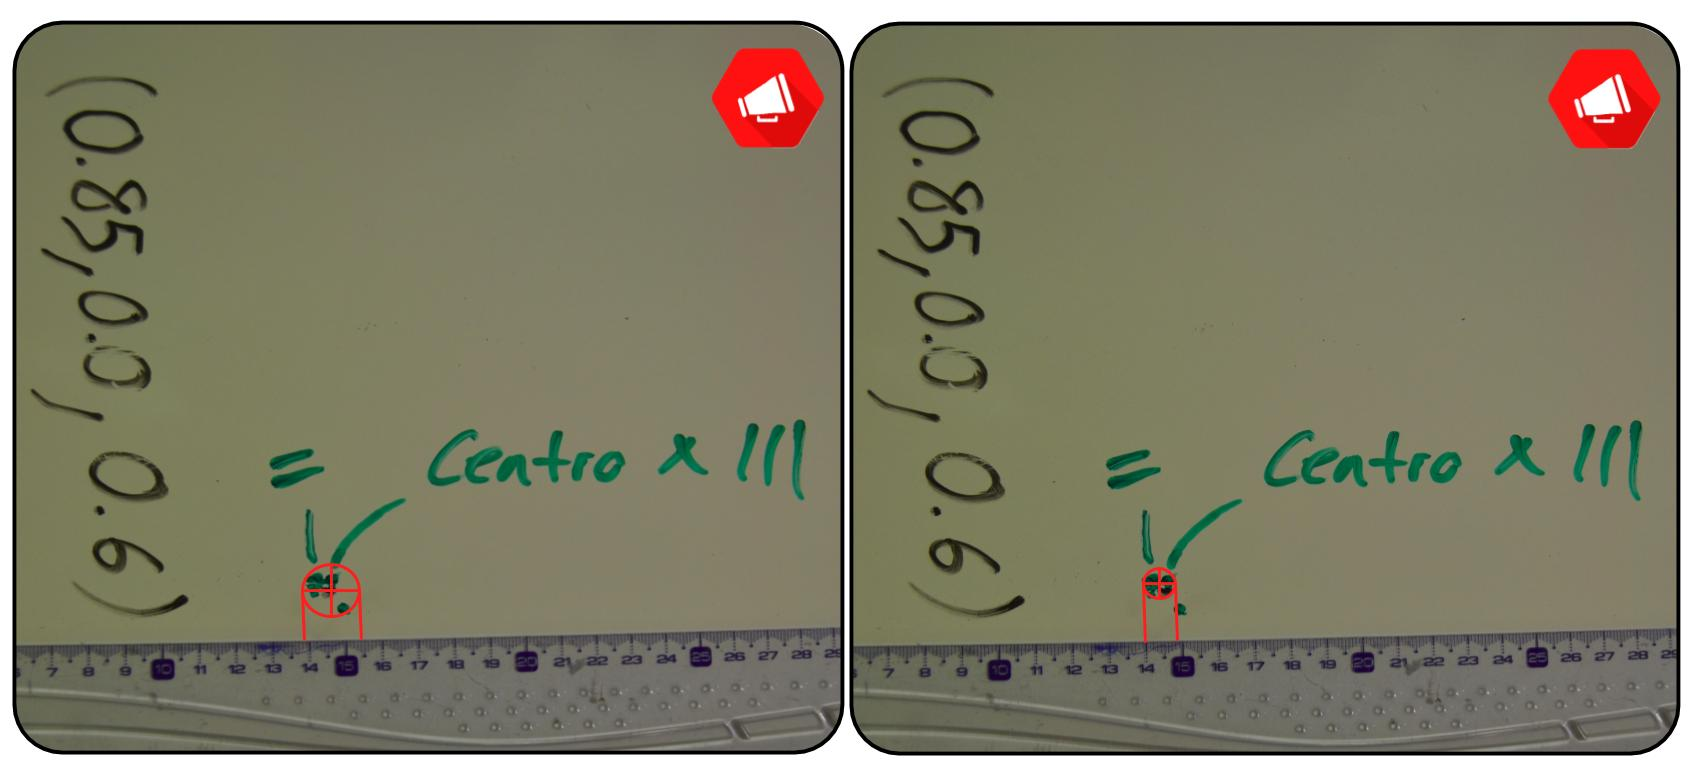
\includegraphics[width=1\textwidth]{figuras/Imagenes_Resultados/pruebas_1.jpg}
		\caption{Pruebas de precisión en (0.85,0.0,0.6)}
		\label{fig:Resultados:prueba1}
		\immagesource{Autor}
	\end{figure}
	
	\begin{figure}[t]
		\centering
		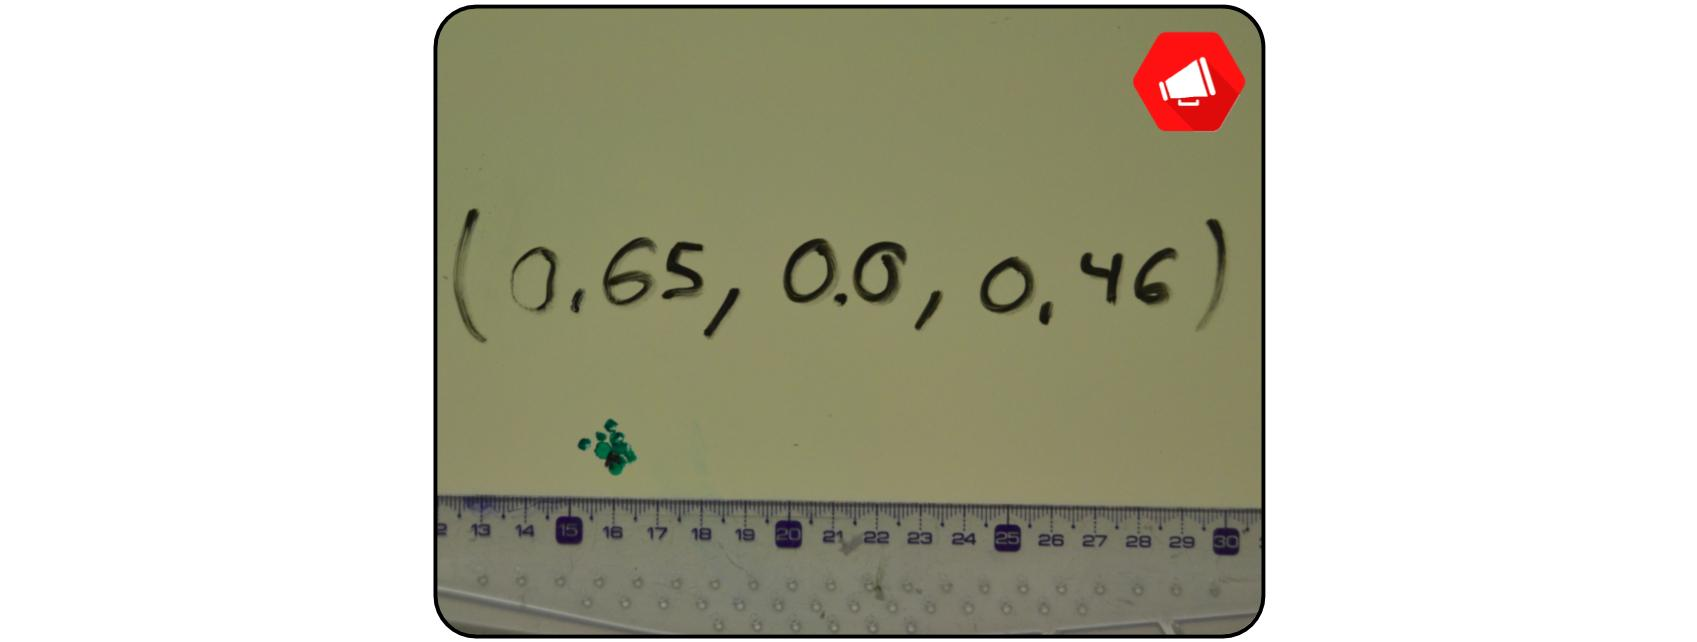
\includegraphics[width=1\textwidth]{figuras/Imagenes_Resultados/pruebas_2.jpg}
		\caption{Pruebas de precisión en (0.65,0.0,0.46)}
		\label{fig:Resultados:prueba2}
		\immagesource{Autor}
	\end{figure}
	
	En la tabla \ref{tab:resultados_precision} pueden verse resumidos los resultados de los test así como la desviación frente a la precisión y repetibilidad observada. Se presentan datos respecto de la desviación máxima primero en precisión, de todos los puntos respecto a la referencia; y segundo respecto a la repetibilidad midiendo la desviación dentro de agrupaciones de puntos. Los datos proporcionados son estimaciones altamente dependientes de la precisión con que se han realizado los test y la limitación del material utilizado.
	\\
	
	Puede apreciarse que, aun habiendo ligeras desviaciones entre grupos de puntos se dan bastantes repeticiones donde los puntos se superponen. 
	\\
	
	Se puede concluir, que aunque la precisión no es muy elevada es suficiente para la aplicación buscada. Además, aun acumulando error en la precisión se puede comprobar que se consigue una repetibilidad más que aceptable.
	
	\begin{table}[htbp]
		\centering
		\caption{Test de precisión del brazo robótico}
		\label{tab:resultados_precision}
		\immagesource{Autor}
		\begin{center}
			\begin{tabular}{|c|c|c|c|}
				\hline
				\textbf{Test} & \textbf{Repeticiones} & \textbf{Precisión} & \textbf{Repetibilidad} \\
				\hline
				1 & 10 & $<$ 4 mm & $<$ 5 mm \\
				\hline
				2 & 9 & $<$ 5 mm  & $<$ 6 mm \\
				\hline
			\end{tabular}
		\end{center}
	\end{table}